%/*% pdflatex -file-line-error -interaction nonstopmode %

\documentclass{article}
\usepackage{graphicx}
\usepackage{amsmath}
\usepackage{amsfonts}
\usepackage{bookmark}
\usepackage{booktabs}
\usepackage{gensymb}
\usepackage{exercises}
\graphicspath{ {./images/3.4} }
\usepackage{indentfirst}
\usepackage{amsthm}
\usepackage{yhmath}
\usepackage{placeins}
\newcommand*{\oldneg}{\mathord{\sim}}
\newcommand\showdiv[1]{\overline{\smash{)}#1}}
\newcommand\Mydiv[1]{%
\smash{\raise.3ex\hbox{$\big)$}}\mkern-8mu
        \overline{\enspace\strut#1}}
\setlength{\tabcolsep}{5pt}
\theoremstyle{definition}
\newtheorem{definition}{Definition}

\setlength{\parindent}{.5in}
\setlength{\parskip}{12pt}
\renewcommand{\arraystretch}{2}

\title{3.4 Answers}
\begin{document}
\maketitle

\section*{1}


Given a function $f(x)$, the definition of the inverse function $f^{-1}$ of $f(x)$ is that every input value $y$ for $f^{-1}(y)$ is such that if 
$f(x)=y$, then $f^{-1}(y)=x$.

\section*{2}


A function $g$ is an inverse of a function $f$ iff $f(g(x))=x$ and $g(f(x))=x$.

\section*{10}
\[ y=-\frac{2}{3}x+2 \]
\[ x=-\frac{2}{3}y+2 \textrm{ (Switch variables)} \]
\[ x-2=-\frac{2}{3}y \]
\[ -\frac{3}{2}x+3=y \]

\section*{11}
\[ y=-\frac{3}{5}x+\frac{7}{5} \]
\[ x=-\frac{3}{5}y+\frac{7}{5} \textrm{ (Switch variables)} \]
\[ x-\frac{7}{5}=-\frac{3}{5}y \]
\[ -\frac{5}{3}x+\frac{7}{3}=y \]

\section*{13}


The error here is that, when switching the variables, $y$ was changed to $-x$, and $-x$ was changed to $y$. Actually, $-x$ should be changed to $-y$, 
and $y$ should be changed to $x$. Thus:
\[ y=-x+3 \]
\[ x=-y+3 \]
\[ x-3=-y \]
\[ -x+3=y \]

\section*{14}
$y=\frac{1}{3}x$

\section*{19}


We need to show that $f(g(x))=x$ and $g(f(x))=x$.
\[ f(g(x))=f(\frac{1}{4}x-\frac{9}{4})=4(\frac{1}{4}x-\frac{9}{4})+9=x-9+9=x \]
and \[ g(f(x))=g(4x+9)=\frac{1}{4}(4x+9)-\frac{9}{4}=x+\frac{9}{4}-\frac{9}{4}=x \]

\section*{20}


We need to show that $f(g(x))=x$ and $g(f(x))=x$.
\[ f(g(x))=f((\frac{x+2}{5})^\frac{1}{2})=5((\frac{x+2}{5})^\frac{1}{2})^2-2=5(\frac{x+2}{5})-2=x+2-2=x \]
and
\[ g(f(x))=g(5x^2-2)=(\frac{5x^2-2+2}{5})^\frac{1}{2}=(\frac{5x^2}{5})^\frac{1}{2}=(x^2)^\frac{1}{2}=x \]

\section*{26}
\[ y=-\frac{2}{5}x^3 \]
\[ x=-\frac{2}{5}y^3 \textrm{ (Switch variables)} \]
\[ -\frac{5}{2}x=y^3 \]
\[ \sqrt[3]{-\frac{5}{2}x}=y \]

\section*{27}
\[ y=\frac{16}{25}x^2,x\le 0 \]
\[ x=\frac{16}{25}y^2 \textrm{ (Switch variables)} \]
\[ \frac{25}{16}x=y^2 \]
\[ \pm\sqrt{\frac{25}{16}x}=y \]
\[ \frac{5}{4}\pm\sqrt{x}=y \]
Because $x\le 0$, we take $-\sqrt{x}$, meaning $f^{-1}=\frac{5}{4}-\sqrt{x}$. 

\section*{28}
\[ y=-\frac{1}{64}x^3 \]
\[ x=-\frac{1}{64}y^3 \]
\[ -64x=y^3 \]
\[ \sqrt[3]{-64x}=y \]
\[ -4\sqrt[3]{x}=y \]
C

\section*{37}
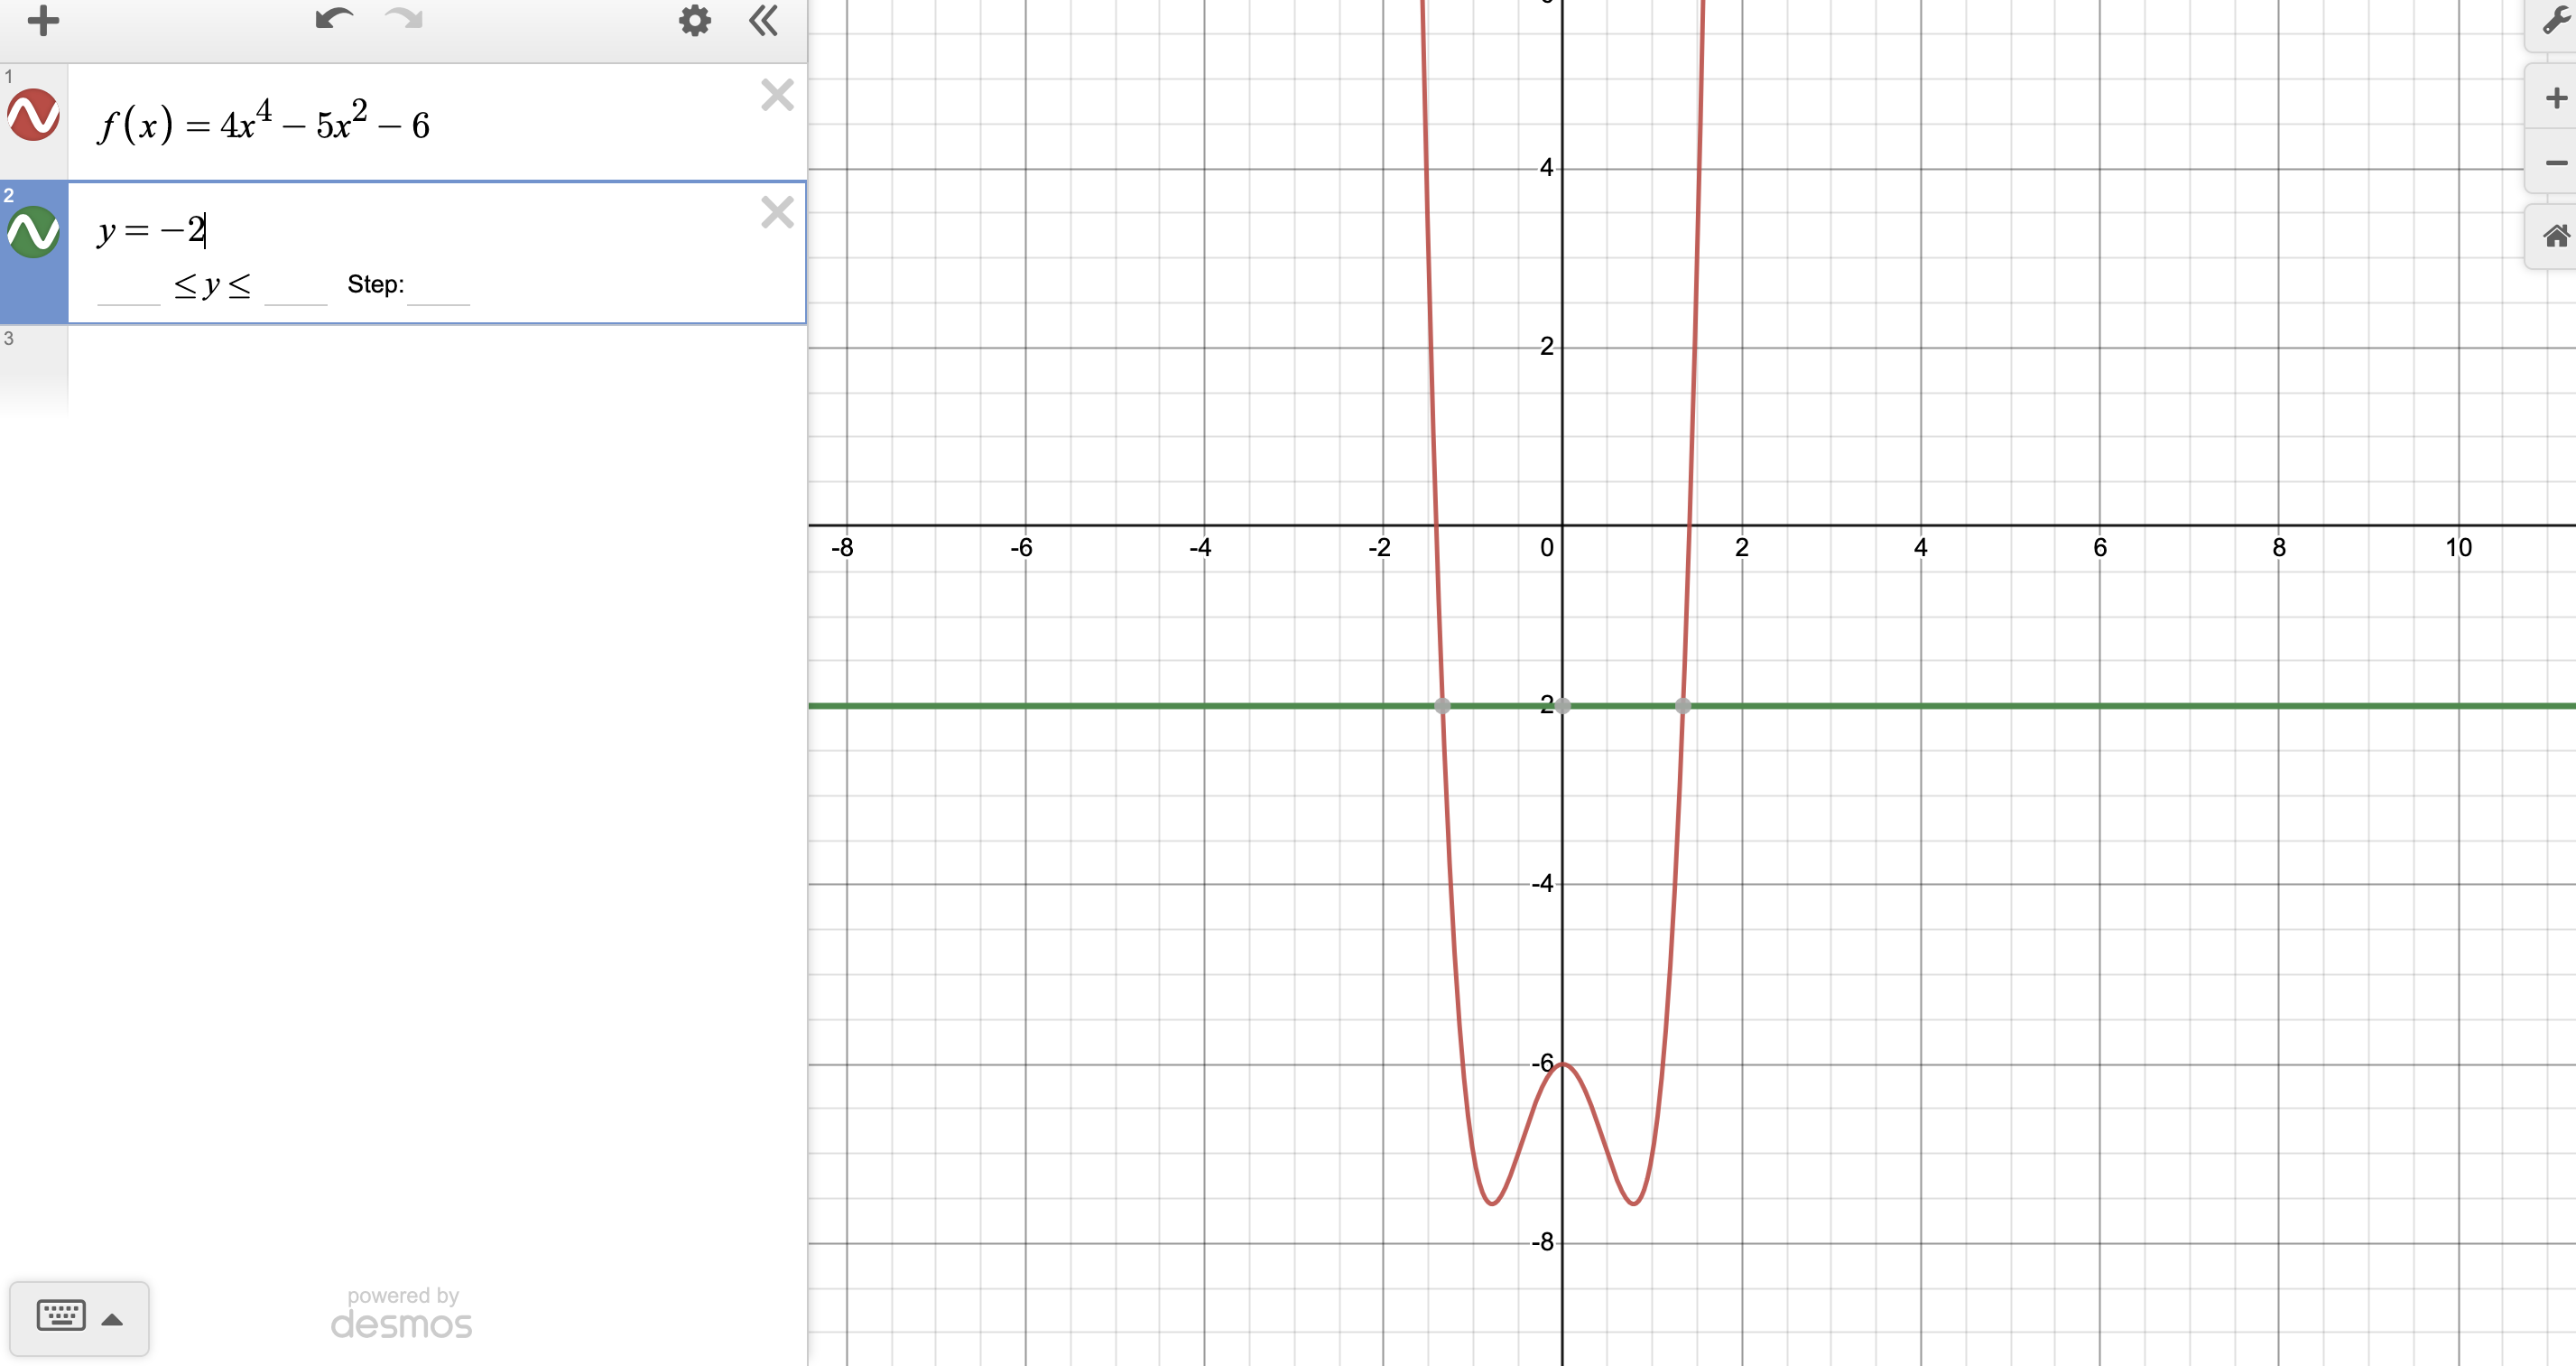
\includegraphics[width = 4in, height = 4in, angle = -90]{37picture}
Because horizontal lines, such as $y=-2$, pass through the graph of $f$ more than once, we know that the inverse of $f$ is not a function.

\section*{42}
\[ y=\frac{2x^3-6}{9} \]
\[ x=\frac{2y^3-6}{9} \]
\[ 9x=2y^3-6 \]
\[ 9x+6=2y^3 \]
\[ \frac{9x+6}{2}=y^3 \]
\[ \sqrt[3]{\frac{9x+6}{2}}=y \]

\section*{43}
\[ y=x^4-9,x\ge 0 \]
\[ x=y^4-9 \]
\[ x+9=y^4 \]
\[ \pm\sqrt[4]{x+9}=y \]
Because $x\ge 0$, we take $+\sqrt[4]{x+9}$, meaning $f^{-1}=+\sqrt[4]{x+9}$.

\section*{44}
(a): This is false because for any positive even integer $n$, if we take the function $f(x)=x^n$, this function has two different inputs 
(namely $\pm\sqrt[n]{y}$) for every output $y$, meaning the inverse function would have two inputs for every output, meaning it is not a function.\newline
(b): This is true because for any positive odd integer $n$, if we take the function $f(x)=x^n$, this function has exactly one input for 
(namely $\sqrt[n]{y}$) for every output $y$, meaning the inverse fucntion would have exactly one input for every output, thus making it a function.

\section*{45}
Consider some linear function $f(x)=mx+b$. Thus, the inverse of this function is:
\[ y=mx+b \]
\[ x=my+b \textrm{ (Switch variables)} \]
\[ x-b=my \]
\[ \frac{x-b}{m}=y \]
\[ \frac{x}{m}-\frac{b}{m}=y \]
This function has a slope of $\frac{1}{m}$, and a $y$-intercept of $-\frac{b}{m}$.

\section*{48}
(a): The inverse of the given model is
\[ C=\frac{5}{9}(F-32) \]
\[ \frac{9}{5}C+32=F \]
This model can, given a value of $C$ (degrees in Celsius), give you a value for the same degrees in Fahrenheit.\newline
(b): At the start of the race, it was $-5\degree C$, and at the end it was $10\degree C$. Thus, at the start of the race, it was: 
$\frac{9}{5}(-5)+32=-9+32=23$ degrees Fahrenheit, and was $\frac{9}{5}(10)+32=18+32=50$ degrees Fahrenheit at the end of the race.\newline
(c): Using a graphing calculator, one can see that the two functions intersect at $-40,-40$.

\section*{49}
We are given that $v=1.34\sqrt{l}$ where $v$ is the maximum hull speed and $l$ is the length (in feet) of the boat's waterline. Because negative lengths 
don't make sense here, we know that $l\ge 0$ is a requirenment. The inverse of this model is:
\[ v=1.34\sqrt{l} \]
\[ \frac{v}{1.34}=\sqrt{l} \]
\[ \pm\sqrt{\frac{v}{1.34}}=l \]
Because $l\ge 0$, this means that we take $+\sqrt{\frac{v}{1.34}}$, meaning $f^{-1}=+\sqrt{\frac{v}{1.34}}$. Thus, the waterline needed to achieve 
a maximum speed of $7.5$ knots is:
\[ +\sqrt{\frac{7.5}{1.34}}=+\sqrt{5.56}\approx 2.36 \]

\end{document}

